\documentclass[conference]{IEEEtran}
\IEEEoverridecommandlockouts
% IEEE ICTAI 2026 submission. Compile on Overleaf with bibtex (IEEEtran style).

\usepackage{cite}
\usepackage{amsmath,amssymb}
\usepackage{graphicx}
\usepackage{booktabs}
\usepackage{multirow}
\usepackage{xcolor}
\usepackage[hidelinks]{hyperref}

\graphicspath{{figures/}}

\begin{document}

\title{StegaQR: Robust Neural Data Embedding in QR Codes\\ with Switchable Channel Modes}

% ICTAI is single-blind; fill author block before camera-ready.
\author{\IEEEauthorblockN{Anonymous Author(s)}
\IEEEauthorblockA{Affiliation \\ City, Country \\ email@domain}}

\maketitle

\begin{abstract}
Quick Response (QR) codes are ubiquitous machine-readable carriers, yet the data
they expose is entirely public. We present StegaQR, a neural method that embeds an
additional private bitstring inside a standard-looking QR code through learned color
perturbations, so that any conventional reader still recovers the public payload
while only a trained decoder recovers the private one. The core of the method is a
spatial bit-grid payload layout, in which each private bit is assigned to one cell of
a grid that is upsampled to the code resolution. We show that this layout makes the
problem learnable at practical payload sizes; the global message-broadcast injection
used by prior neural data-hiding methods stalls near chance. StegaQR supports three switchable embedding modes (per-channel,
cross-channel, and a QR-anchored hybrid that leaves the structural modules
untouched) and couples the learned channel with error-correction coding. Training
the encoder and decoder end to end through a differentiable distortion layer yields
robustness that transfers to physical capture. Across five seeds, distortion-trained
models recover the full private message with 99 to 100 percent success under
simulated degradation, and recover it from every one of ten real photographs of a
displayed code, while the public payload remains 100 percent standard-decodable. We
characterize the operating frontier between imperceptibility and robustness and
report a classical baseline that fails under the same conditions.
\end{abstract}

\begin{IEEEkeywords}
QR codes, information hiding, data embedding, deep learning, robust watermarking,
error-correction coding, screen-shooting robustness.
\end{IEEEkeywords}

\section{Introduction}
A QR code carries a single public payload that any camera can read. That openness
drives its use in ticketing, payments, and product labeling, but it also means the
code cannot carry anything that should travel with the artifact and stay out of reach
of an ordinary scanner. A second, private channel that rides inside the same
printed or displayed code would support uses such as tamper evidence, device-pairing
secrets, and provenance tags, provided two conditions hold. A standard reader must
still decode the public payload, and the private channel must survive the way QR codes
are actually consumed, which is by photographing them from paper or a screen.

Two bodies of work come close, but each leaves a gap. Neural data-hiding methods learn
an encoder and decoder jointly and can embed a bitstring that survives printing and
re-photography~\cite{baluja2017hiding,zhu2018hidden,tancik2020stegastamp,bui2023rosteals}.
They hide data inside natural photographs, however, so the recovered medium is the photo
rather than a still-scannable code. Methods that hide data specifically inside QR codes
do keep a public level readable, but they are classical: they substitute textured
patterns or multiplex color channels by hand, and the high-capacity color variants need a
dedicated decoder, so the composite code is no longer a standard
QR~\cite{tkachenko2016twolevel,yang2018hiq,chu2013halftone}. None of the QR-specific
methods is learned, and their robustness to the screen-to-camera channel is largely
untested.

We present StegaQR, a method that bridges these two lines. A convolutional encoder takes
a standard QR code and a private bitstring and outputs a stego code that differs from the
original only by a learned color perturbation. A convolutional decoder recovers the
private bits from the stego code, while any conventional reader recovers the public
payload unchanged. The encoder and decoder are trained end to end through a differentiable
distortion layer that simulates the photometric and geometric corruptions of capture. This
training is the source of the learned channel's robustness.

The design choice that makes this work at useful payload sizes is how the private bits
enter the network. Prior neural hiders broadcast the message as a constant signal over
the whole image and read it back by global pooling. We instead lay the bits out
spatially. Each bit occupies one cell of a grid that is upsampled to the code resolution,
and the decoder pools its activation map back to the same grid to read each cell. Because
a single shared convolution then learns one write-and-read operation that applies to
every cell, learning a 100-bit code becomes about as hard as learning a handful of bits.
Under an identical training budget, the spatial layout reaches 100 percent bit accuracy
at 100 bits, while the broadcast layout stays near 52 percent, which is chance.

StegaQR exposes three switchable embedding modes that trade fault isolation, capacity,
and structural guarantees. A segregated mode uses independent per-channel sub-networks, a
cross-channel mode uses all three color channels jointly, and a QR-anchored hybrid masks
the perturbation off the finder, timing, and format modules so the structural anatomy of
the code is provably unchanged. On top of the learned channel we apply error-correction
coding, which turns the decoder's high but imperfect bit accuracy into exact message
recovery. The need for distortion-aware training is concrete. Machine-learning decoders
for printed or displayed 2D barcodes are brittle to real photometric and environmental
variation, because a captured code depends heavily on the device and lighting, and a
decoder trained for one setting often fails in another~\cite{xie2020lcac}. Training
through the distortion layer removes this brittleness, and we confirm the result on real
captures rather than on simulation alone.

Because the embedding strength is a tunable knob, StegaQR spans an operating frontier. At
high peak signal-to-noise ratio (PSNR) the perturbation is not visible to a human and the
embedding is genuinely covert. At the lower PSNR needed to survive physical capture the
perturbation appears as a faint color tint, so we describe that regime as robust data
embedding rather than as human-imperceptible steganography. We characterize both ends and
state the trade-off plainly.

This paper makes the following contributions.
\begin{itemize}
\item A neural method that embeds an arbitrary private bitstring inside a
standard-decodable QR code by learned color perturbation, distinct from hiding data in
natural images and from classical QR data hiding.
\item A spatial bit-grid payload layout, with an ablation showing it is the component
that makes the problem learnable at 100 bits (100 percent versus 52 percent for global
broadcast).
\item Three switchable embedding modes, including a QR-anchored hybrid that leaves the
structural modules untouched, compared across five seeds.
\item A distortion-trained, error-correction-coded channel characterized along the
imperceptibility, robustness, and capacity axes, with a classical baseline for reference.
\item Validation on real screen-to-camera capture, where the private message is recovered
from every test photograph while the public payload stays fully standard-decodable.
\end{itemize}

\section{Related Work}

\subsection{Neural data hiding in images}
Deep data hiding trains an encoder and a decoder as a pair. Baluja hid a full color
image inside a same-size cover and recovered it with a companion
network~\cite{baluja2017hiding}. HiDDeN moved to bitstring payloads and introduced the
now-standard recipe of inserting a differentiable noise layer between encoder and
decoder, so the system learns robustness to blur, cropping, and an approximation of
JPEG~\cite{zhu2018hidden}. StegaStamp carried this to the physical world: it embeds a
hyperlink bitstring into a natural photograph that stays decodable after the photo is
printed and re-captured, using simulated printing and reimaging during training and a
BCH code to clean up residual bit errors~\cite{tancik2020stegastamp}. RoSteALS placed
the payload as a single offset in the latent space of a pretrained
autoencoder~\cite{bui2023rosteals}, and RivaGAN added attention and adversarial critics
for video~\cite{zhang2019rivagan}. Two properties separate all of these from our setting.
The cover is a natural image, so the artifact that must stay useful is a photograph
rather than a scannable code, and the payload is injected by broadcasting the message
across the whole image and reading it back with global pooling, with no spatial
correspondence between a bit and a location.

\subsection{Data hiding inside QR codes}
A separate line keeps the QR code itself as the carrier. The two-level QR code stores a
public level identical to a standard QR, readable by any application, and a private level
formed by replacing black modules with textured patterns that are recovered by pattern
correlation and Reed-Solomon decoding~\cite{tkachenko2016twolevel}. High-capacity color
QR codes such as HiQ superpose several monochrome codes into one color symbol, which
raises capacity but needs a trained classifier to separate the channels, so the result is
no longer a standard monochrome QR~\cite{yang2018hiq}. Halftone QR codes embed a visible
image into the code by splitting each module into a three-by-three block and binding only
the center submodule to the decoded value~\cite{chu2013halftone}. Anti-copying 2D barcodes
embed authentication information in the print noise itself~\cite{xie2020lcac}. These
methods preserve or extend QR functionality, but they are hand-designed rather than
learned, and where capacity is highest the public readability is lost. Their behavior
under the screen-to-camera channel is largely unreported.

\subsection{Robustness to the physical channel}
Robustness to printing and re-photography, and to the related screen-shooting channel in
which a displayed image is captured by a camera, has become its own topic. Fang et al.
characterized the screen-shooting channel through lens deformation, light-source
deformation, and moire, and embedded the watermark redundantly at small scale to survive
it~\cite{fang2019screen}. PIMoG showed that a noise layer modeling only the dominant
distortions, namely perspective, illumination, and moire, is enough to train a deep
watermarking network end to end and reach high screen-shooting
accuracy~\cite{fang2022pimog}. We adopt the same principle of a differentiable distortion
layer during training and apply it to a QR cover.

\subsection{Positioning}
StegaQR sits at an intersection that none of these occupy. It is a learned encoder and
decoder, like the neural image hiders, but its cover is a QR code that remains
standard-decodable, like the classical QR methods. It lays the payload out spatially
rather than broadcasting it, exposes switchable embedding modes including one that
provably preserves the structural modules, and is validated on real screen-to-camera
capture. The closest neighbors are StegaStamp, which is neural and physical but hides in
natural images with a broadcast payload, and the two-level QR code, which keeps the public
payload but is classical and untested on the capture channel we target.
Table~\ref{tab:related} summarizes these contrasts.

\begin{table*}[t]
\centering
\caption{StegaQR against representative prior work. ``Public QR'' is whether a standard
monochrome QR reader still decodes the public payload from the published artifact. Payload
figures are as reported by each source: HiDDeN $52$ bits at $0.203$ bits per pixel;
StegaStamp $56$ bits after BCH correction; 2LQR up to $20{,}000$ private bits in a
version-40 symbol; HiQ up to $8{,}900$ bytes across three color layers. ``ML dec.'' marks a
classical embedding read back by a trained classifier rather than a learned encoder and
decoder pair. Dashes mark properties the source does not report; ``n/a'' marks the public-QR
column for natural-image covers.}
\label{tab:related}
\begin{tabular}{llllllc}
\toprule
Method & Cover & Learned & Payload & Imperceptibility & Robustness validated & Public QR \\
\midrule
Baluja~\cite{baluja2017hiding}         & natural image & yes      & full RGB image                 & high               & none                         & n/a \\
HiDDeN~\cite{zhu2018hidden}            & natural image & yes      & $52$ b ($0.203$ bpp)           & visually indist.   & simulated                    & n/a \\
StegaStamp~\cite{tancik2020stegastamp} & natural photo & yes      & $56$ b (post-BCH)              & near-invisible     & print + photo                & n/a \\
RoSteALS~\cite{bui2023rosteals}        & natural image & yes      & $100$ b                        & high               & simulated                    & n/a \\
2LQR~\cite{tkachenko2016twolevel}      & QR            & no       & up to $20{,}000$ b             & visible (textured) & print-scan                   & yes \\
HiQ~\cite{yang2018hiq}                 & color QR      & ML dec.  & up to $8{,}900$ B              & overt color        & mobile capture               & no  \\
Halftone QR~\cite{chu2013halftone}     & QR            & no       & visible image                  & overt              & ---                          & yes \\
\midrule
\textbf{StegaQR (ours)}                & QR            & yes      & $100$ b raw, $33$--$56$ b net  & $18$--$55$ dB (tunable) & simulated + screen-to-camera & yes \\
\bottomrule
\end{tabular}
\end{table*}

\section{Method}

\begin{figure*}[t]
\centering
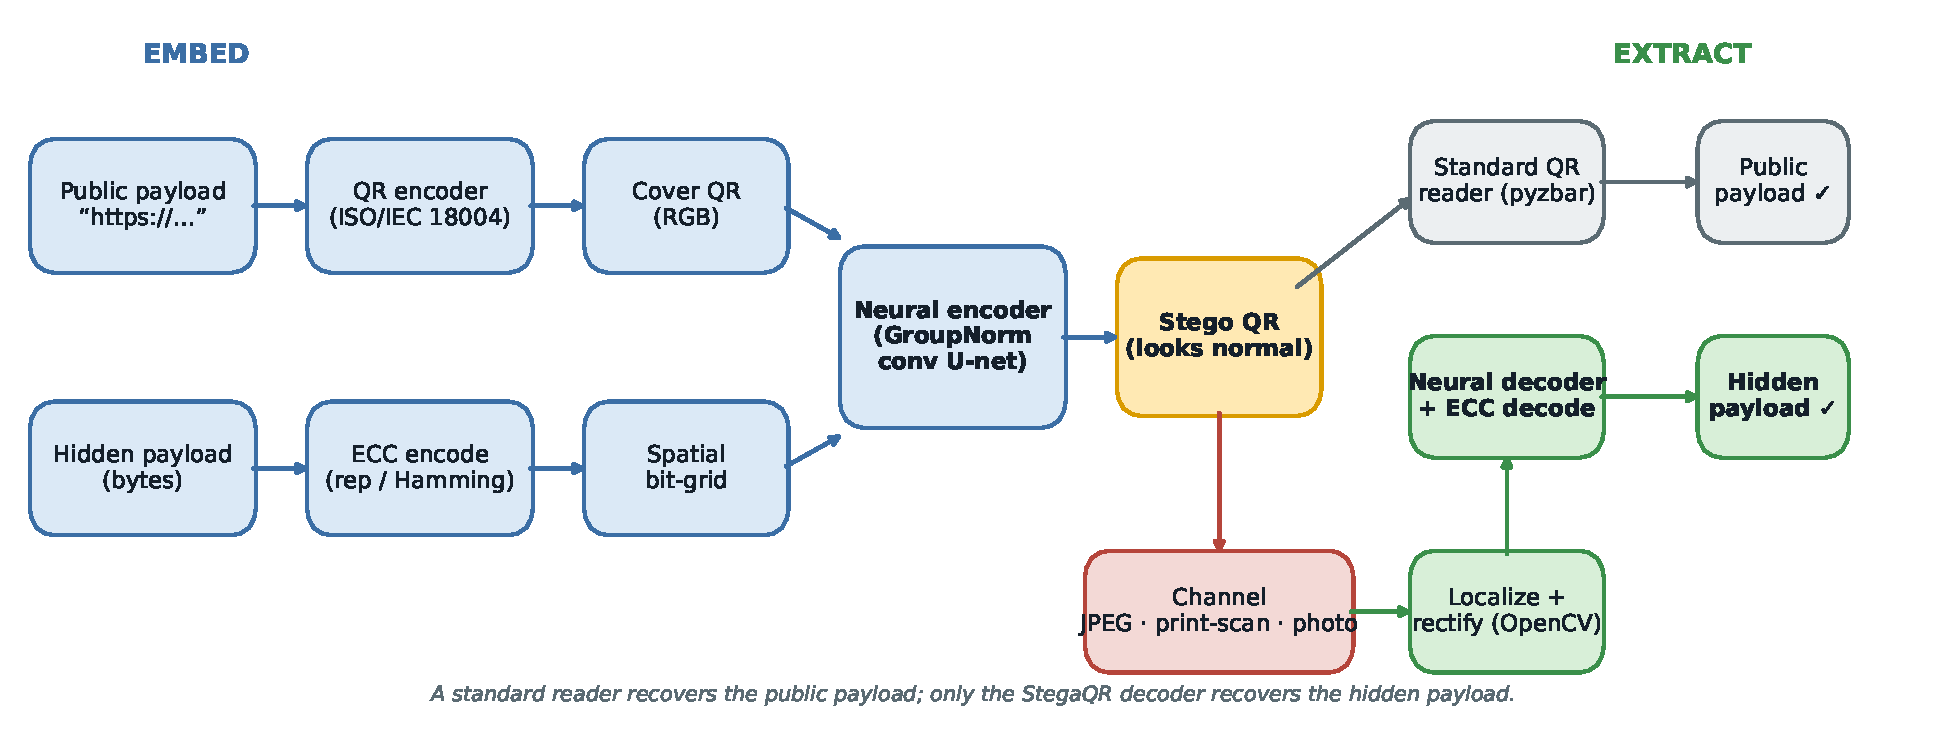
\includegraphics[width=0.95\textwidth]{fig_system}
\caption{StegaQR pipeline. The public payload is rendered as a standard QR cover; the
private bitstring is error-correction coded, laid out on a spatial bit-grid, and fused
with the cover by a convolutional encoder that outputs a bounded color perturbation. A
standard reader recovers the public payload from the stego code, while the trained
decoder recovers the private bits. Encoder and decoder are trained jointly through a
differentiable distortion layer.}
\label{fig:system}
\end{figure*}

\subsection{Overview}
StegaQR turns a public payload and a private bitstring into a single stego QR image
(Fig.~\ref{fig:system}). The public payload is rendered as a standard QR code that serves
as the cover. The private bitstring is protected by an error-correcting code, arranged on
a spatial grid, and fused with the cover by a convolutional encoder that outputs a bounded
color perturbation. At extraction, a standard reader recovers the public payload from the
stego image directly, while a convolutional decoder recovers the private bits. The encoder
and decoder are trained jointly with a differentiable distortion layer placed between them.

\subsection{Cover and payload representation}
\textbf{Cover.} The public payload is encoded as a version-4 QR code with error-correction
level M under ISO/IEC 18004~\cite{iso18004}, which gives a $33\times33$ module grid. Each
module is rendered as a square of $m$ pixels, so the cover is an RGB image of side $33m$;
we use $m=4$. Dark modules are black and light modules are white.

\textbf{Payload.} The private message is first expanded by an error-correcting code
(Section~\ref{ssec:ecc}) into $L$ coded bits. We place these bits on a square grid. Let
$g=\lceil\sqrt{L}\,\rceil$. The bits fill a $g\times g$ grid, one bit per cell, and the
grid is upsampled by nearest-neighbor interpolation to the cover resolution to form a
single-channel bit map $B\in\{0,1\}^{H\times W}$. Each bit thus occupies a contiguous
block of pixels at a fixed location.

\subsection{Spatial bit-grid}
\label{ssec:bitgrid}
The bit map is the reason the task becomes learnable. A convolution is translation equivariant
with shared weights, so a network that learns to write one cell has learned to write every
cell, and likewise for reading. Embedding $L$ bits is then about as hard as embedding a
few. This is the point of departure from the global broadcast used by prior neural
hiders~\cite{zhu2018hidden,tancik2020stegastamp,bui2023rosteals}, which replicate the
message uniformly over the image and read it back by global pooling; there the network
must learn $L$ distinct global patterns, which does not scale to the payload sizes we need.
Section~\ref{ssec:ablation} quantifies the gap. Figure~\ref{fig:bitgrid} shows the write
and read paths.

\begin{figure*}[t]
\centering
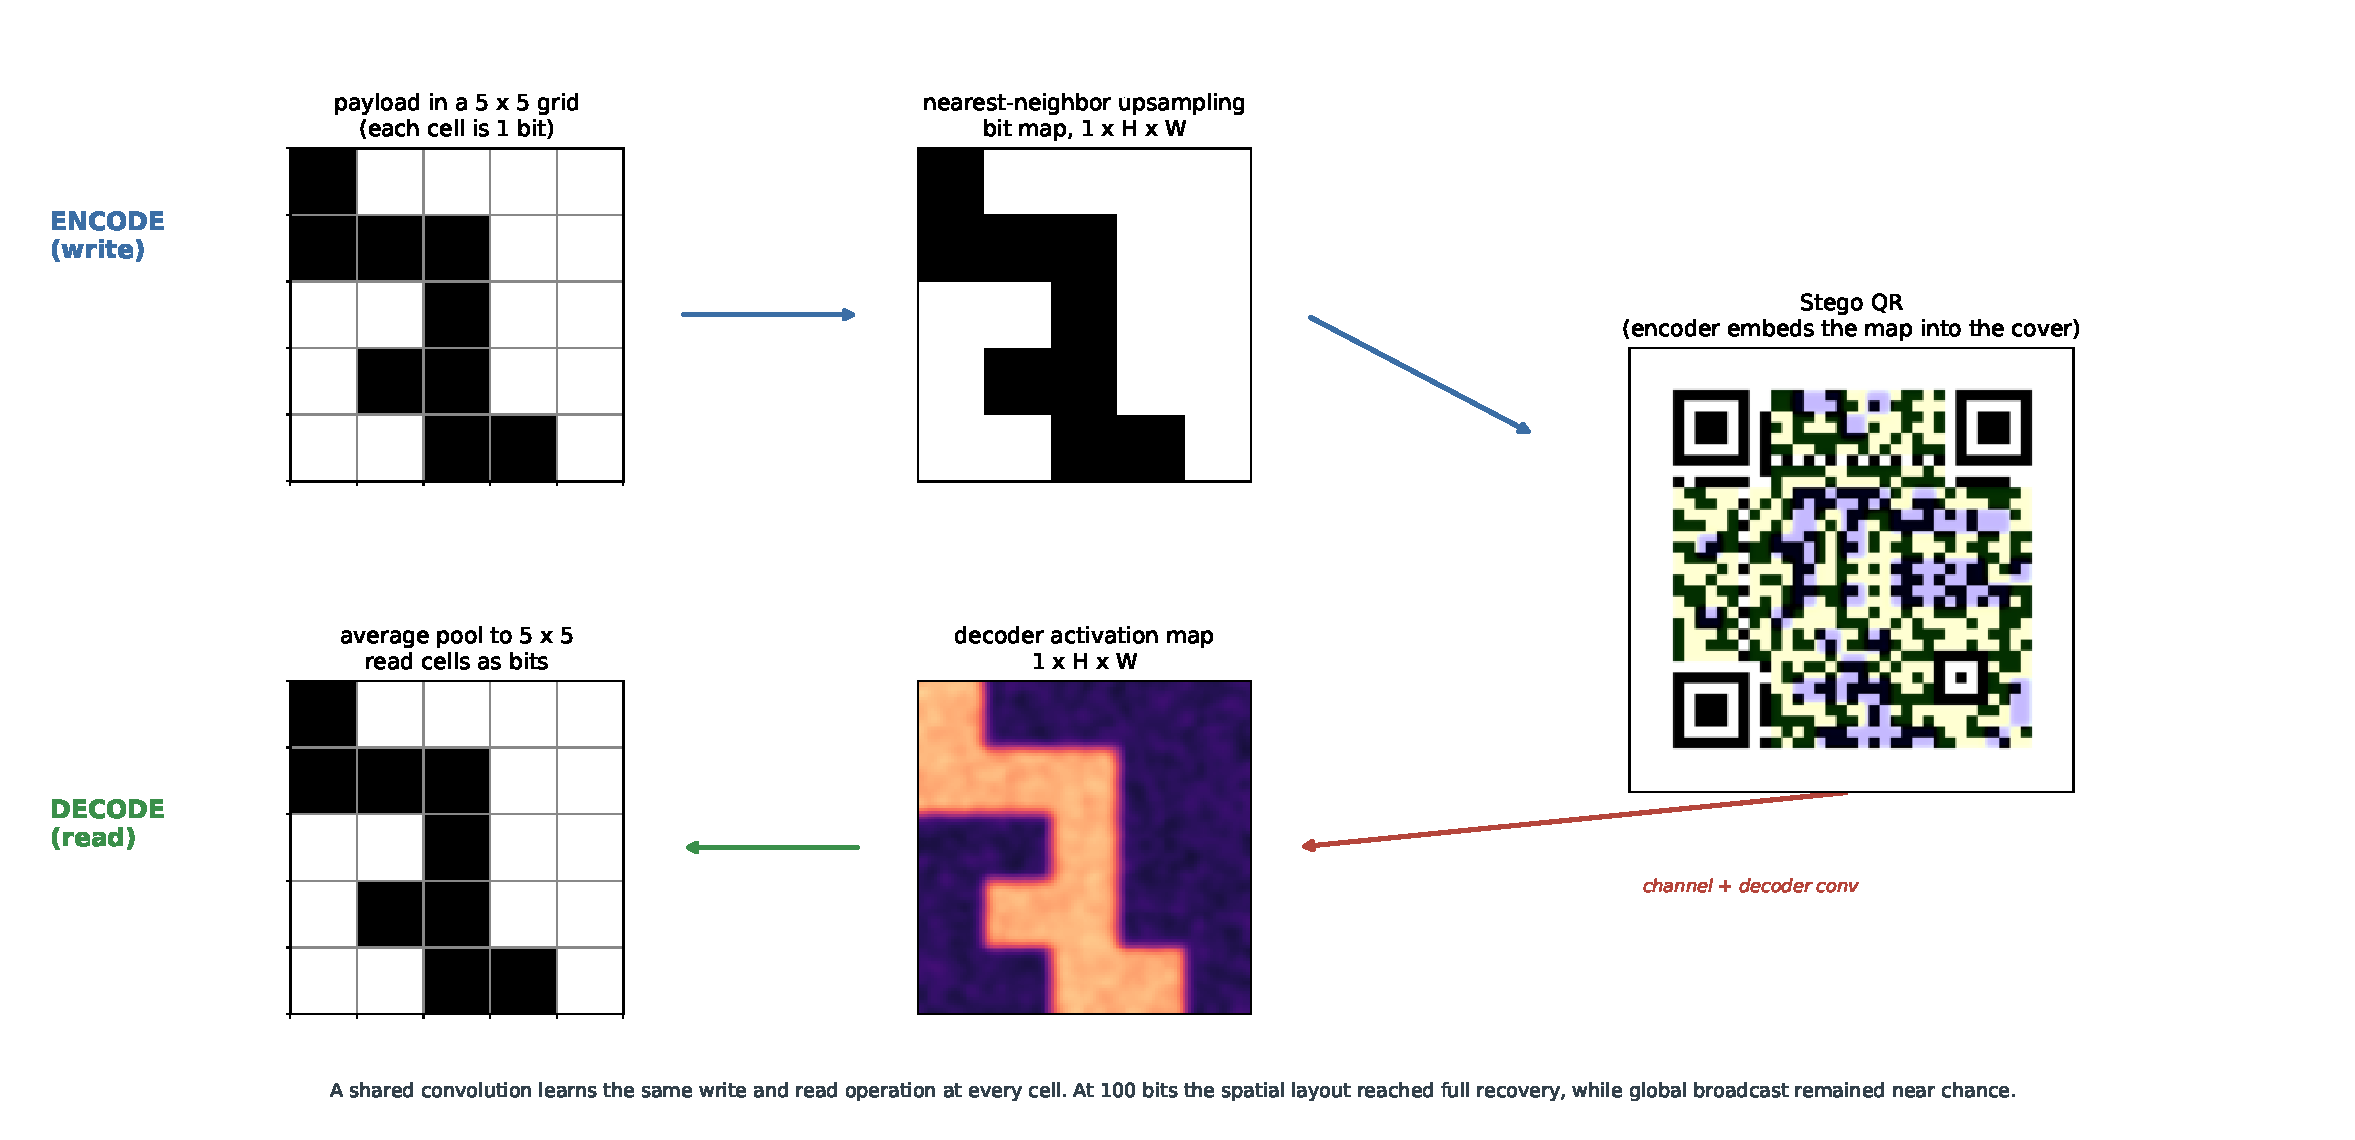
\includegraphics[width=0.95\textwidth]{fig_bitgrid}
\caption{Spatial bit-grid. On embedding (top) the payload fills a $g\times g$ grid, one
bit per cell, upsampled to the code resolution and written into the cover by the encoder.
On extraction (bottom) the decoder produces an activation map, average-pools it back to the
grid, and reads each cell. A single shared convolution learns one write-and-read operation
that applies to all cells.}
\label{fig:bitgrid}
\end{figure*}

\subsection{Encoder and decoder}
\textbf{Encoder.} The encoder receives the concatenation of the cover, the bit map, and,
in the hybrid mode, a structural mask (Section~\ref{ssec:modes}). It applies five
$3\times3$ convolutional blocks with 64 channels, each block being convolution, group
normalization, and ReLU with a residual connection, followed by a $1\times1$ convolution
to three channels and a $\tanh$ nonlinearity. The output is scaled by a perturbation bound
$\varepsilon$, added to the cover, and clamped:
\begin{equation}
\hat{x} = \mathrm{clip}\!\big(x + \varepsilon\,\tanh(f_\theta(x,B)),\,0,\,1\big).
\end{equation}
The bound $\varepsilon$ is the single knob that trades imperceptibility against robustness.

\textbf{Decoder.} The decoder applies six convolutional blocks to the stego image, a
$1\times1$ convolution to a single-channel activation map, an adaptive average pool to the
$g\times g$ grid, and a per-cell readout that yields $L$ logits. Thresholding gives the
recovered coded bits, which the error-correcting code maps back to the message. The
architecture is shown in Fig.~\ref{fig:arch}.

\textbf{Normalization.} We use group normalization rather than batch normalization. In the
robust regime the perturbation is small relative to the cover, and the running statistics
that batch normalization accumulates during training do not match the per-batch statistics
seen at inference, which collapses decoding at test time. Group normalization removes this
train and test mismatch.

\begin{figure*}[t]
\centering
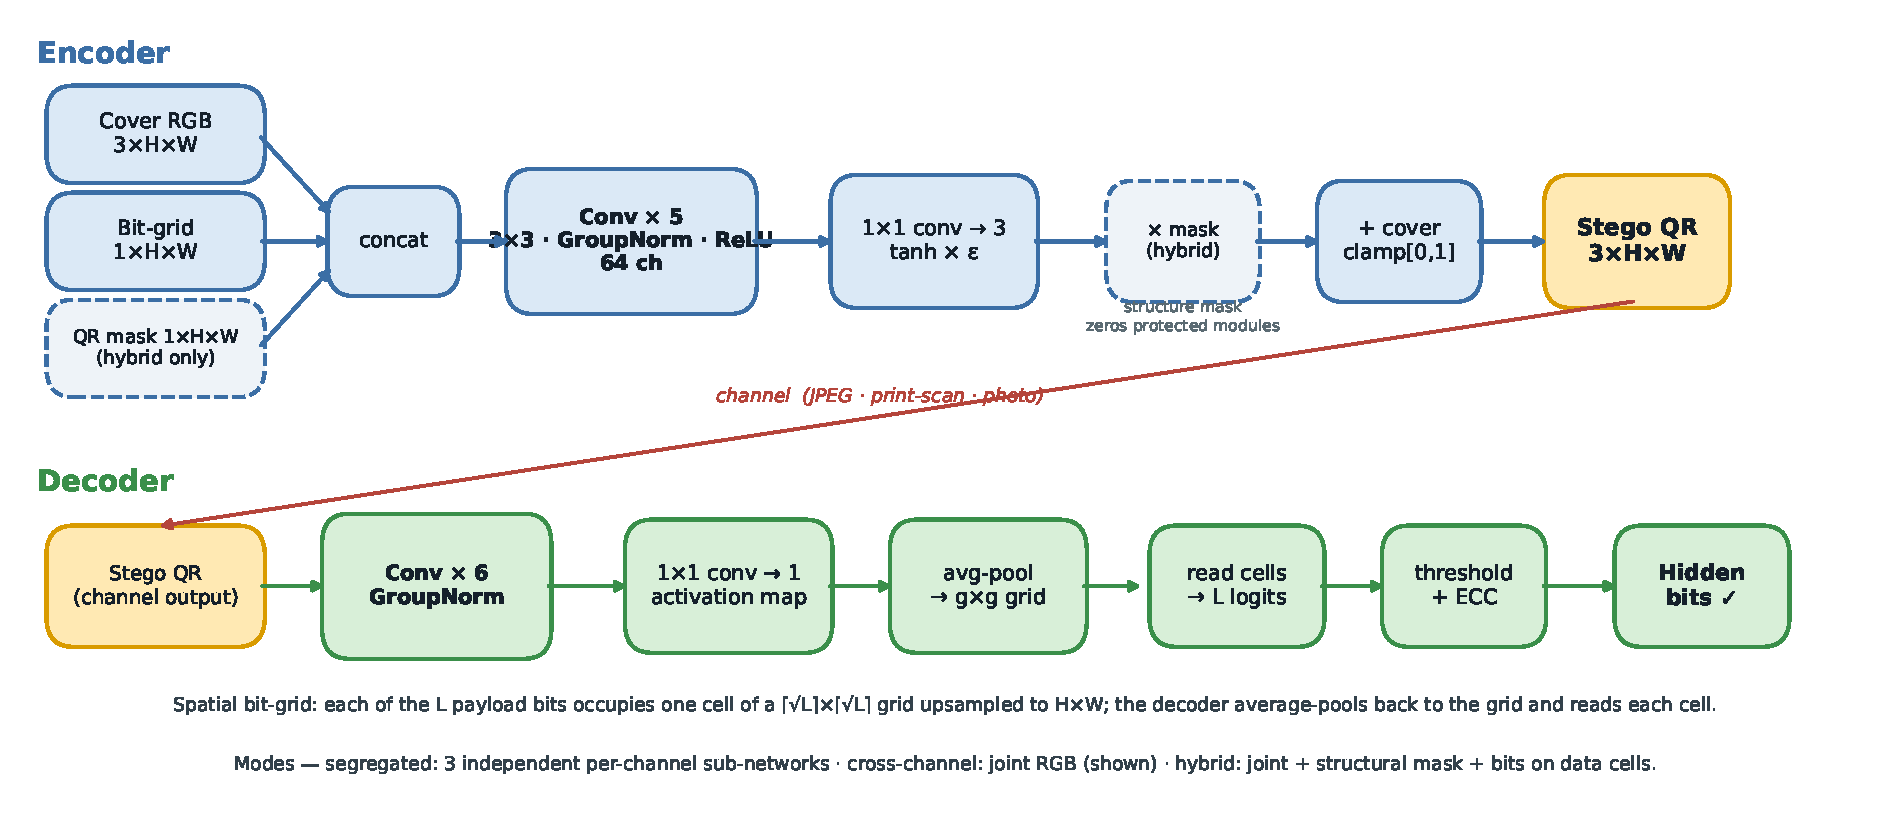
\includegraphics[width=0.95\textwidth]{fig_architecture}
\caption{Encoder and decoder. The encoder fuses the cover, the bit-grid map, and (hybrid
only) the structural mask through grouped convolutions and emits a bounded, optionally
masked perturbation added to the cover. The decoder reads the payload by pooling its
activation map back to the bit-grid. Group normalization is used throughout.}
\label{fig:arch}
\end{figure*}

\subsection{Channel modes}
\label{ssec:modes}
The three modes share the template above but differ in how color is used and what is
protected.

\textbf{Segregated.} Three independent sub-encoders and sub-decoders, one per color
channel, each embedding $L/3$ bits on its own grid. A failure in one channel cannot
corrupt the others, which gives fault isolation at the cost of treating the channels
separately.

\textbf{Cross-channel.} A single encoder and decoder use all three channels jointly, which
gives the most freedom in placing the perturbation.

\textbf{Hybrid (QR-anchored).} The cross-channel design with two QR-aware constraints. A
binary structural mask marks the finder, timing, format, and alignment modules, and the
encoder multiplies its perturbation by this mask so those modules are left exactly as in
the cover, which guarantees the structural anatomy of the code is unchanged. Because masked
cells cannot carry payload, the hybrid layout places bits only on the data-rich cells of a
finer grid, selected once from the mask. We found that an explicit color-calibration branch
in the decoder destabilized training without improving accuracy, so the hybrid decoder
omits it; the convolutional decoder already absorbs photometric variation.

\subsection{Distortion layer and training}
\textbf{Distortion layer.} A differentiable distortion layer sits between the encoder and
decoder during training and applies, each with a fixed probability, additive Gaussian
noise, a JPEG-like quantization proxy, brightness scaling, per-channel color shift, and
Gaussian blur. The decoder therefore learns to read bits from degraded stego images, and
that ability carries over to physical capture.

\textbf{Objective.} The loss combines a decoding term, an imperceptibility term, and a
structural term:
\begin{equation}
\mathcal{L} = \lambda_d\,\mathcal{L}_{\text{dec}} + \lambda_p\,\mathcal{L}_{\text{perc}}
            + \lambda_s\,\mathcal{L}_{\text{struct}}.
\end{equation}
$\mathcal{L}_{\text{dec}}$ is the binary cross-entropy between recovered and true coded
bits. $\mathcal{L}_{\text{perc}}$ combines mean squared error with a penalty on the largest
per-pixel deviation, keeping the perturbation small. $\mathcal{L}_{\text{struct}}$ is a
hinge that keeps structural modules close to their cover values.

\textbf{Curriculum.} Optimizing the decoding and imperceptibility terms together from
scratch is unstable: the imperceptibility term can drive the perturbation to zero before
the decoder has learned to read it. We therefore train decoding only for a short warmup,
then ramp the imperceptibility and structural weights linearly to their targets. The
networks are optimized with Adam at a base rate of $10^{-3}$ under cosine annealing with
gradient clipping. We select the final checkpoint by its message recovery under distortion,
breaking ties toward higher PSNR, which avoids both the trivial high-PSNR solution that
fails under capture and an over-strong perturbation that is needlessly visible.

\subsection{Error-correction coding}
\label{ssec:ecc}
The decoder recovers individual bits with high but imperfect accuracy, and one wrong bit
ruins a message. We therefore protect the message with an error-correcting code before
embedding. We use a repetition code with soft-decision combining, in which the decoder sums
the logits of the repeated copies, and a Hamming(7,4) code as a higher-rate alternative.
With $k$ message bits expanded to $L$ coded bits, the net capacity is $k$ and the rate is
$k/L$. Coding converts the decoder's per-bit accuracy into exact message recovery at the
cost of capacity.

\section{Experimental Setup}
\textbf{Data.} Training data is generated on the fly. Each sample is a version-4,
level-M QR code rendered from a random alphanumeric public payload, paired with a random
private message. No external dataset is used. Unless stated otherwise the payload is
$L=100$ coded bits and the module size is $m=4$, giving a $132\times132$ cover.

\textbf{Training.} Each configuration is trained for five seeds. We train for 24 epochs
with batch size 16, 1500 fresh samples per epoch, Adam at $10^{-3}$ with cosine
annealing and gradient clipping, a three-epoch decode-only warmup, and an eight-epoch
ramp of the imperceptibility and structural weights. We compare two regimes: a clean
regime with the distortion layer disabled, and a distortion-trained regime with it
enabled. Unless noted, the perturbation bound is $\varepsilon=0.3$ and the encoder
adapts the actual perturbation downward through the imperceptibility loss.

\textbf{Metrics.} We report bit accuracy (fraction of correct coded bits), full-decode
rate (fraction of samples with every coded bit correct), message-decode rate (fraction
of messages recovered exactly after error correction), PSNR and SSIM of the stego image
against the cover, and public decode rate, the fraction of stego images whose public
payload a standard reader (ZBar) decodes correctly. Rates are reported as mean and a 95
percent confidence interval over the five seeds.

\textbf{Hardware.} All experiments run on a single 16~GB GPU.

\section{Results}

\subsection{Channel modes and the effect of distortion training}
Table~\ref{tab:modes} reports the three modes under both training regimes. Two patterns
are consistent across seeds. First, the public payload is decoded by a standard reader in
every condition, so the embedding never breaks the cover. Second, distortion training
produces the robustness. Clean-trained models are near perfect on clean stego images but
recover the full message from only about 10 to 14 percent of distorted images, whereas
distortion-trained models recover it from 99 to 100 percent. Cross-channel and segregated
behave almost identically; the hybrid mode matches them at a slightly higher PSNR, because
restricting the perturbation to data modules concentrates it where it is useful.

\begin{table*}[t]
\centering
\caption{Channel modes, capacity 100 bits, five seeds (mean $\pm$ 95\% CI). FDR is the
full-decode rate (all bits correct). PSNR/SSIM are stego vs. cover. Public decode is by a
standard ZBar reader.}
\label{tab:modes}
\begin{tabular}{llcccccc}
\toprule
Mode & Training & Clean bit-acc & Clean FDR & Dist.\ bit-acc & Dist.\ FDR & PSNR (dB) & Public decode \\
\midrule
\multirow{2}{*}{Segregated}    & clean      & $100.0\pm0.0$ & $100.0\pm0.0$ & $65.5\pm5.7$  & $13.9\pm11.3$ & $63.5$ & $100.0$ \\
                               & distortion & $100.0\pm0.0$ & $99.8\pm0.3$  & $100.0\pm0.0$ & $99.1\pm0.8$  & $17.6$ & $100.0$ \\
\multirow{2}{*}{Cross-channel} & clean      & $100.0\pm0.0$ & $99.5\pm0.9$  & $63.8\pm10.6$ & $10.0\pm19.6$ & $61.7$ & $100.0$ \\
                               & distortion & $100.0\pm0.0$ & $99.8\pm0.3$  & $100.0\pm0.0$ & $99.2\pm1.5$  & $19.0$ & $100.0$ \\
\multirow{2}{*}{Hybrid}        & clean      & $100.0\pm0.0$ & $99.8\pm0.3$  & $66.1\pm7.1$  & $13.9\pm11.3$ & $58.8$ & $100.0$ \\
                               & distortion & $100.0\pm0.0$ & $100.0\pm0.0$ & $100.0\pm0.0$ & $100.0\pm0.0$ & $22.3$ & $100.0$ \\
\bottomrule
\end{tabular}
\end{table*}

\subsection{The spatial bit-grid is the enabling component}
\label{ssec:ablation}
To isolate the bit-grid, we replace it with the global broadcast used by prior neural
hiders and train both under an identical budget. At 100 bits
the spatial grid reaches 100 percent bit accuracy and 100 percent full-decode, clean and
distorted, while the broadcast layout stays at 51 to 53 percent bit accuracy, at chance
level, and never achieves a single full decode. At this payload size the grid is therefore
a prerequisite for learning rather than a refinement of it.

\subsection{Imperceptibility and robustness form a tunable frontier}
The perturbation bound $\varepsilon$ moves the system along a frontier
(Fig.~\ref{fig:imperceptibility}). At small $\varepsilon$ the stego code is visually
indistinguishable from the cover. A clean-trained cross-channel model reaches $54.9$~dB
PSNR with SSIM $1.000$ and full public decode, which is the covert regime
(Fig.~\ref{fig:examples}, second column). Surviving physical capture requires a larger
perturbation, which appears as a faint color tint at PSNR near $20$~dB; this is the robust
regime that we use for the capture study. Figure~\ref{fig:examples} also shows that the
hybrid residual is exactly zero on the finder patterns, confirming that the structural
modules are untouched.

\begin{figure}[t]
\centering

\includegraphics[width=\columnwidth]{fig_imperceptibility}
\caption{Imperceptibility against robustness across trained models. The covert regime
(high PSNR) is near invisible; the robust regime (lower PSNR) survives capture.}
\label{fig:imperceptibility}
\end{figure}

\begin{figure*}[t]
\centering
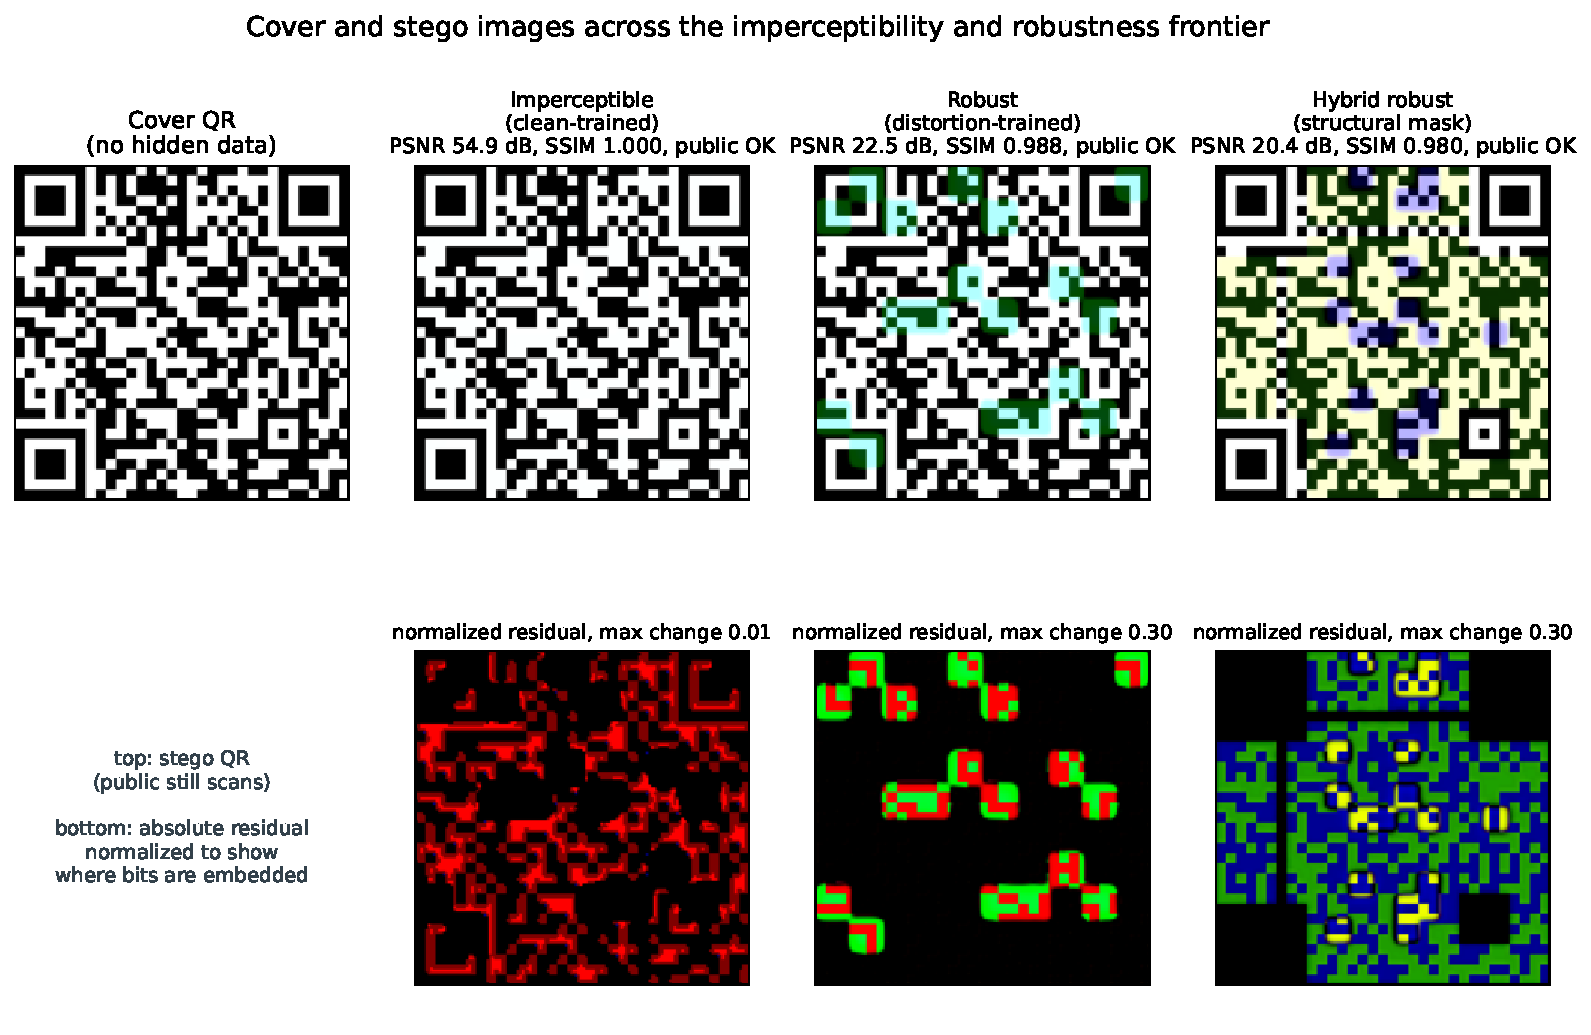
\includegraphics[width=0.96\textwidth]{fig_examples}
\caption{Cover versus stego at three operating points with normalized residuals. The
covert model is visually identical to the cover at $54.9$~dB; the robust and hybrid models
carry a faint tint. The hybrid residual is zero on the finder patterns (bottom right),
showing the structural mask leaves them unchanged. All public payloads decode.}
\label{fig:examples}
\end{figure*}

\subsection{Capacity scaling}
Table~\ref{tab:capacity} sweeps the embedded capacity of the cross-channel model under
distortion. Distorted bit accuracy stays at or above 99 percent from 25 to 200 bits, and
the full-decode rate stays high except at 150 bits, where one seed was an outlier and
widened the interval. Higher capacity is therefore available, with the usual caveat that
exact full-message decode at large payloads benefits from error correction.

\begin{table}[t]
\centering
\caption{Capacity scaling, cross-channel, distortion-trained.}
\label{tab:capacity}
\begin{tabular}{cccc}
\toprule
Capacity (bits) & Dist.\ bit-acc & Dist.\ FDR & PSNR (dB) \\
\midrule
25  & $99.9\pm0.1$  & $97.7\pm2.3$  & $23.7$ \\
50  & $100.0\pm0.0$ & $99.7\pm0.5$  & $20.3$ \\
100 & $100.0\pm0.0$ & $99.2\pm1.5$  & $19.0$ \\
150 & $99.3\pm1.4$  & $86.5\pm24.2$ & $23.9$ \\
200 & $100.0\pm0.0$ & $95.3\pm7.0$  & $19.0$ \\
\bottomrule
\end{tabular}
\end{table}

\subsection{Error-correction coding gives exact messages}
A single wrong bit ruins a message, so we measure message-decode rate after coding
(Table~\ref{tab:ecc}). On the distortion-trained cross-channel model, a Hamming(7,4) code
recovers the message exactly in every case at 56 net bits, and a rate-1/3 repetition code
reaches $99.5$ percent at 33 net bits. Coding cleanly converts the decoder's high bit
accuracy into exact recovery.

\begin{table}[t]
\centering
\caption{Message-decode rate under distortion (cross-channel, 100 embedded bits).}
\label{tab:ecc}
\begin{tabular}{lccc}
\toprule
Code & Net bits & Rate & Message decode \\
\midrule
None (raw)    & 100 & $1.00$ & $99.2\pm1.5$ \\
Repetition-3  & 33  & $0.33$ & $99.5\pm0.6$ \\
Repetition-5  & 20  & $0.20$ & $98.1\pm1.1$ \\
Hamming(7,4)  & 56  & $0.57$ & $100.0\pm0.0$ \\
\bottomrule
\end{tabular}
\end{table}

\subsection{Classical baseline}
A classical per-channel least-significant-bit scheme embeds the same payload with no
training. It is perfect on clean images, at 100 percent full-decode and $78$~dB PSNR, but
collapses under the distortion layer to $53.8$ percent bit accuracy and $3.9$ percent
full-decode. The learned, distortion-trained channel closes this gap.

\subsection{Real screen-to-camera capture}
The simulated distortion layer is a stand-in for the physical channel, so we test on real
captures. We displayed ten distinct stego codes from the distortion-trained hybrid model
on a monitor and photographed them with a smartphone, free-hand, at varied angle and
distance. Each photograph was localized and rectified with a standard detector, then
decoded. The QR was located in all ten, the public payload decoded in all ten, and the
private message, protected by a rate-1/3 code, was recovered in all ten
(Fig.~\ref{fig:capture}). The robustness learned against the simulated layer therefore
transfers to genuine display, optics, and sensor distortions.

\begin{figure*}[t]
\centering
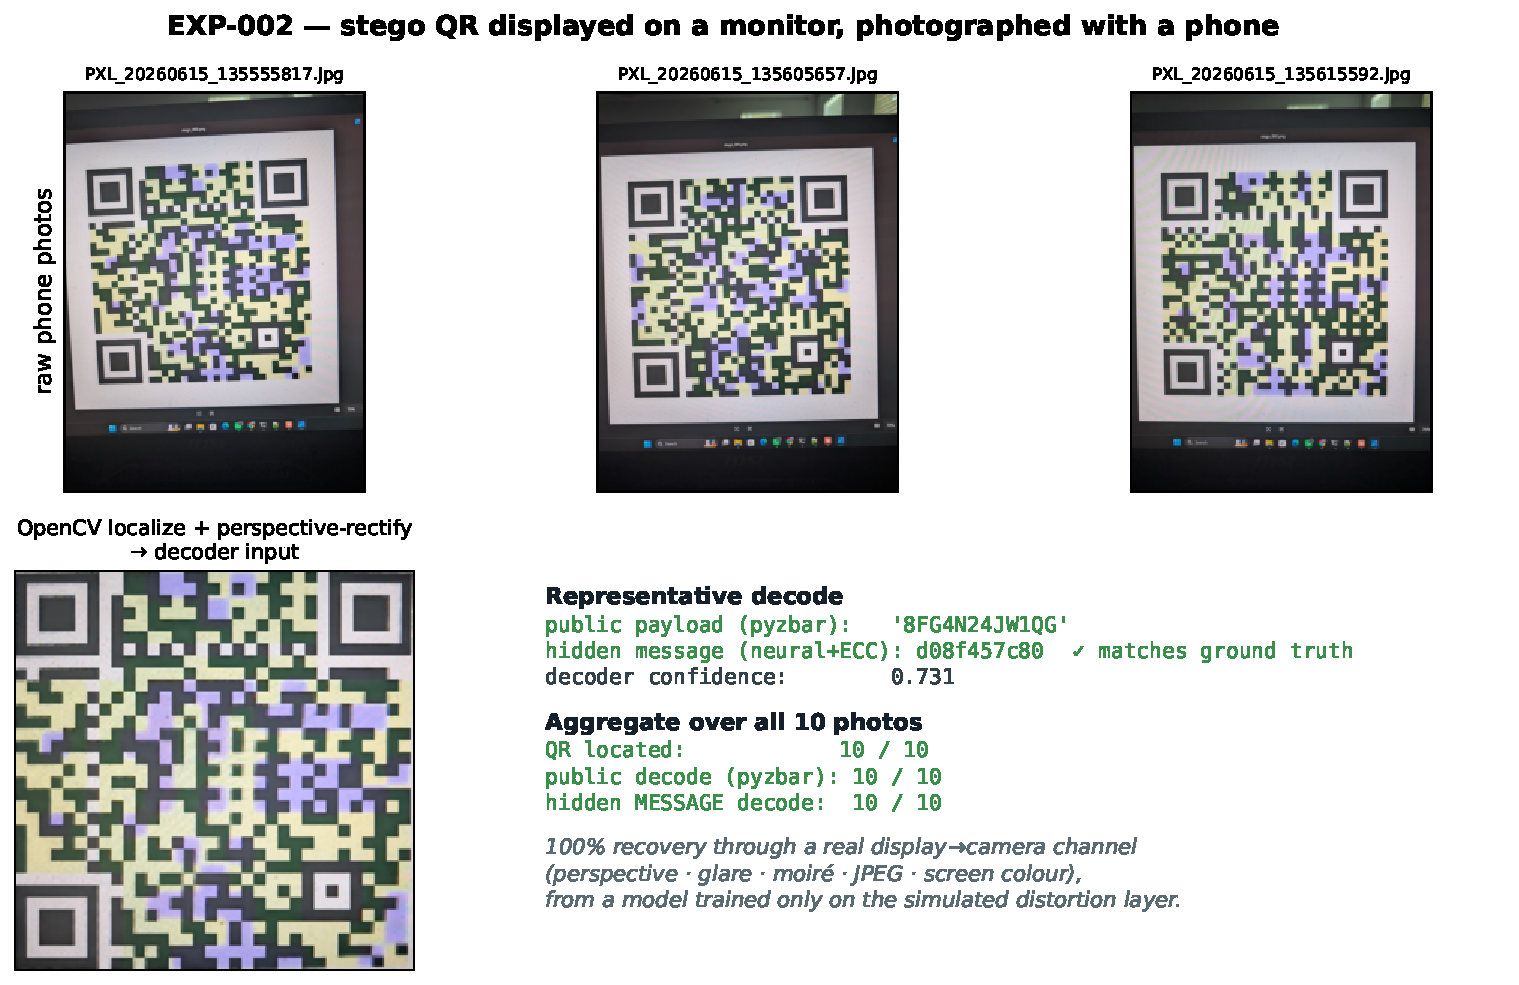
\includegraphics[width=0.96\textwidth]{fig_capture}
\caption{Real screen-to-camera capture. Stego codes displayed on a monitor and
photographed with a smartphone are localized, rectified, and decoded. Across ten photos
the public payload and the private message are recovered in every case.}
\label{fig:capture}
\end{figure*}

\section{Discussion and Limitations}
The frontier makes the main limitation explicit: the covert regime, where
the perturbation is invisible, does not survive physical capture, and the regime that
survives capture carries a faint but visible color tint. We therefore present the visible
robust regime as robust data embedding rather than as human-imperceptible steganography,
and reserve the covert label for the high-PSNR end. A reader who looks closely can tell a
robust StegaQR code from a plain one; what they cannot do is read the private payload.

Net capacity is modest. At 100 embedded bits a rate-1/3 code leaves 33 message bits, and a
Hamming code leaves 56, which is enough for an identifier, a short token, or a key but not
for a long message. The capacity sweep shows that the embedded budget extends to at least
200 bits at high bit accuracy, so larger payloads are reachable, though exact recovery at
the top of that range leans more on the error-correcting code.

The evaluation fixes the QR version, error-correction level, and resolution, and the
physical study is a single session on one display and one camera with ten codes. These
choices are enough to establish that distortion training transfers to real capture, but a
broader sweep over devices, lighting, angle, and printed media, and over QR versions, would
strengthen the deployment case. We also do not study steganalysis: we do not measure how
hard it is for an adversary who knows the scheme to detect or remove the payload. In the
covert regime detectability is the natural next question, and in the robust regime the
relevant question is removal under adversarial post-processing.

Finally, the hybrid mode needed care to train. The structural mask removes payload capacity
from the protected cells, and an explicit calibration branch we initially included made the
cold start unstable. Placing bits only on data-rich cells and removing that branch resolved
both, but it shows that QR-aware constraints interact with optimization in ways that a plain
image-hiding setup does not face.

\section{Conclusion}
We presented StegaQR, a learned method that embeds a private bitstring inside a
standard-decodable QR code through a bounded color perturbation. The design rests on a
spatial bit-grid that gives each bit a location, which lets a single shared
convolution learn the embedding at useful payload sizes where the global broadcast of prior
neural hiders stalls at chance. Three switchable modes offer different balances of fault
isolation, capacity, and structural preservation, and a QR-anchored hybrid leaves the
structural modules provably untouched. Training end to end through a differentiable distortion layer, and coupling the
channel with error correction, yields models that recover the full private message from 99
to 100 percent of distorted images and from every one of ten real photographs of a
displayed code, while a standard reader recovers the public payload in every case. The
gains over a clean-trained model and a classical baseline are large, and the imperceptibility
and robustness ends of the system are characterized as a single tunable frontier. Code and
trained models will be released. Future work includes larger payloads, a broader physical
and cross-device study, coverage of more QR versions, and a steganalysis of both regimes.

\bibliographystyle{IEEEtran}
\bibliography{refs}

\end{document}
